%%%%%%%%%%%%%%%%%%%%%%%%%%%%%%%%%%%%%%%%%%%%%%%%%%%%%%%%%%
\begin{frame}
  \begin{center}
    {\Large Introduction to Pandas}
	
	% (Ref: Python for Data Analysis - Katia Oleinik )
  \end{center}
\end{frame}

%%%%%%%%%%%%%%%%%%%%%%%%%%%%%%%%%%%%%%%%%%%%%%%%%%%%%%%%%%
\begin{frame}[fragile]\frametitle{Pandas}
\begin{itemize}
\item Pandas is an open-source Python Library 
\item Providing high-performance data manipulation and analysis. 
\item The name Pandas is derived from the word Panel Data.
\end{itemize}
\end{frame}

%%%%%%%%%%%%%%%%%%%%%%%%%%%%%%%%%%%%%%%%%%%%%%%%%%%%%%%%%%
\begin{frame}[fragile]\frametitle{Key Features of Pandas}
\begin{itemize}
\item Fast and efficient DataFrame object 
\item Default and customized indexing.
\item Tools for loading data into in-memory data objects from different file formats.
\item Handling of missing data.
\item Label-based slicing of large data sets.
\end{itemize}
\end{frame}


%%%%%%%%%%%%%%%%%%%%%%%%%%%%%%%%%%%%%%%%%%%%%%%%%%%%%%%%%%
\begin{frame}[fragile]\frametitle{Data Structures of Pandas}
\begin{itemize}
\item 
    Series: 1D indexed array, size immutable.
    \item 
    DataFrame: General 2D indexed, size-mutable tabular structure with potentially heterogeneously typed columns.
    \item 
    Panel: General 3D indexed, size-mutable array.

\end{itemize}
\end{frame}

%%%%%%%%%%%%%%%%%%%%%%%%%%%%%%%%%%%%%%%%%%%%%%%%%%%%%%%%%%
\begin{frame}[fragile]\frametitle{Series}
Series is a one-dimensional array like structure with homogeneous data. For example, the following series is a collection of integers 10, 23, 56, \ldots
\begin{center}
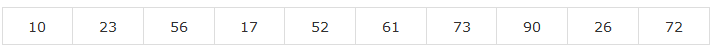
\includegraphics[width=\linewidth,keepaspectratio]{pd1}
\end{center}
\begin{itemize}
\item  Homogeneous data
\item  Size Immutable
\item    Values of Data Mutable
\end{itemize}
\end{frame}

%%%%%%%%%%%%%%%%%%%%%%%%%%%%%%%%%%%%%%%%%%%%%%%%%%%%%%%%%%
\begin{frame}[fragile]\frametitle{DataFrame}
DataFrame is a two-dimensional array with heterogeneous data. For example,
\begin{center}
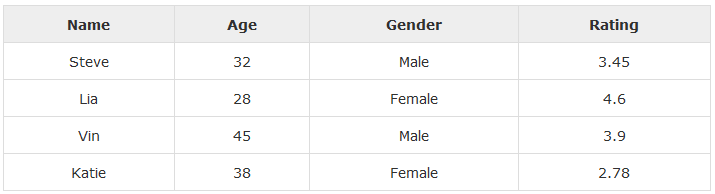
\includegraphics[width=\linewidth,keepaspectratio]{pd2}
\end{center}
\begin{itemize}
\item  Heterogeneous  data
\item  Size Mutable
\item    Values of Data Mutable
\end{itemize}
\end{frame}


%%%%%%%%%%%%%%%%%%%%%%%%%%%%%%%%%%%%%%%%%%%%%%%%%%%%%%%%%%
\begin{frame}[fragile]\frametitle{Pandas}	
\textbf{Series} and \textbf{DataFrame}, both of which are built on top of NumPy.
\begin{lstlisting}
import pandas as pd
import numpy as np
import matplotlib.pyplot as plt
pd.set_option('max_columns', 50)
\end{lstlisting}
\end{frame}

%%%%%%%%%%%%%%%%%%%%%%%%%%%%%%%%%%%%%%%%%%%%%%%%%%%%%%%%%%
\begin{frame}[fragile]\frametitle{Series}
Capable of holding any data type (integers, strings, floating point numbers, Python objects, etc.). 

\begin{lstlisting}
# create a Series with an arbitrary list
s = pd.Series([7, 'Heisenberg', 3.14, -1789710578,     'Happy Eating!'])
print(s)
\end{lstlisting}

\begin{lstlisting}
0                7
1       Heisenberg
2             3.14
3      -1789710578
4    Happy Eating!
dtype: object
\end{lstlisting}
\end{frame}

%%%%%%%%%%%%%%%%%%%%%%%%%%%%%%%%%%%%%%%%%%%%%%%%%%%%%%%%%%%%%%%%%%%%%%%%
\begin{frame}[fragile]
Alternatively, you can specify an index to use when creating the Series.
\begin{lstlisting}
s = pd.Series([7, 'Heisenberg', 3.14, -1789710578, 
   'Happy Eating!'],
index=['A', 'Z', 'C', 'Y', 'E'])
print(s)
\end{lstlisting}
\begin{lstlisting}
A                7
Z       Heisenberg
C             3.14
Y      -1789710578
E    Happy Eating!
dtype: object
\end{lstlisting}
\end{frame}

%%%%%%%%%%%%%%%%%%%%%%%%%%%%%%%%%%%%%%%%%%%%%%%%%%%%%%%%%%%%%%%%%%%%%%%%
\begin{frame}[fragile]\frametitle{Series}		
The Series constructor can convert a dictionary as well, using the keys of the dictionary as its index.
\begin{lstlisting}
d = {'Chicago': 1000, 'New York': 1300, 'Portland': 900, 'San Francisco': 1100,'Austin': 450, 'Boston': None}
cities = pd.Series(d)
print(cities)

Austin            450
Boston            NaN
Chicago          1000
New York         1300
Portland          900
San Francisco    1100
dtype: float64
\end{lstlisting}
\end{frame}

%%%%%%%%%%%%%%%%%%%%%%%%%%%%%%%%%%%%%%%%%%%%%%%%%%%%%%%%%%%%%%%%%%%%%%%%
\begin{frame}[fragile]\frametitle{Series}		
You can use the index to select specific items from the Series 
\begin{lstlisting}
print(cities['Chicago'])

1000.0
\end{lstlisting}

\begin{lstlisting}
print(cities[['Chicago', 'Portland', 'San Francisco']])

Chicago          1000
Portland          900
San Francisco    1100
dtype: float64
\end{lstlisting}
\end{frame}

%%%%%%%%%%%%%%%%%%%%%%%%%%%%%%%%%%%%%%%%%%%%%%%%%%%%%%%%%%%%%%%%%%%%%%%%
\begin{frame}[fragile]\frametitle{Series}		
You can use \textbf{\textit{Boolean indexing}} for selection.
\begin{lstlisting}
print(cities[cities < 1000])

Austin      450
Portland    900
dtype: float64
\end{lstlisting}
\end{frame}

%%%%%%%%%%%%%%%%%%%%%%%%%%%%%%%%%%%%%%%%%%%%%%%%%%%%%%%%%%%%%%%%%%%%%%%%%
%\begin{frame}[fragile]
%That last one might be a little strange, so let's make it more clear - \texttt{cities < 1000} returns a Series of \texttt{True/False} values, which we then pass to our Series cities, returning the corresponding \texttt{True} items.
%\end{frame}

%%%%%%%%%%%%%%%%%%%%%%%%%%%%%%%%%%%%%%%%%%%%%%%%%%%%%%%%%%%%%%%%%%%%%%%%
\begin{frame}[fragile]
\begin{lstlisting}
less_than_1000 = cities < 1000
print(less_than_1000)
print('\n')
print(cities[less_than_1000])

Austin            True
Boston           False
Chicago          False
New York         False
Portland          True
San Francisco    False
dtype: bool

Austin      450
Portland    900
dtype: float64
\end{lstlisting}
\end{frame}

%%%%%%%%%%%%%%%%%%%%%%%%%%%%%%%%%%%%%%%%%%%%%%%%%%%%%%%%%%%%%%%%%%%%%%%%
\begin{frame}[fragile]
You can also change the values in a Series on the fly.
\begin{lstlisting}
# changing based on the index
print('Old value:', cities['Chicago'])
cities['Chicago'] = 1400
print('New value:', cities['Chicago'])

Old value: 1000.0
New value: 1400.0
\end{lstlisting}
\end{frame}

%%%%%%%%%%%%%%%%%%%%%%%%%%%%%%%%%%%%%%%%%%%%%%%%%%%%%%%%%%%%%%%%%%%%%%%%
\begin{frame}[fragile]	
Changing values using boolean logic
\begin{lstlisting}
print(cities[cities < 1000])
print( '\n')
cities[cities < 1000] = 750
print(cities[cities < 1000])

Austin      450
Portland    900
dtype: float64

Austin      750
Portland    750
dtype: float64
\end{lstlisting}
\end{frame}

%%%%%%%%%%%%%%%%%%%%%%%%%%%%%%%%%%%%%%%%%%%%%%%%%%%%%%%%%%%%%%%%%%%%%%%%
\begin{frame}[fragile]\frametitle{Working with Series}
What if you aren't sure whether an item is in the Series? You can check using idiomatic Python.
\begin{lstlisting}
print 'Seattle' in cities
print 'San Francisco' in cities
False
True
\end{lstlisting}
\end{frame}

%%%%%%%%%%%%%%%%%%%%%%%%%%%%%%%%%%%%%%%%%%%%%%%%%%%%%%%%%%%%%%%%%%%%%%%%
\begin{frame}[fragile]
Mathematical operations can be done using scalars and functions.
\begin{lstlisting}
# divide city values by 3
print(cities / 3)

Austin           250.000000
Boston                  NaN
Chicago          466.666667
New York         433.333333
Portland         250.000000
San Francisco    366.666667
dtype: float64
\end{lstlisting}
\end{frame}

%%%%%%%%%%%%%%%%%%%%%%%%%%%%%%%%%%%%%%%%%%%%%%%%%%%%%%%%%%%%%%%%%%%%%%%%%
%\begin{frame}[fragile]
%\begin{lstlisting}
%# square city values
%print(np.square(cities))
%
%Austin            562500
%Boston               NaN
%Chicago          1960000
%New York         1690000
%Portland          562500
%San Francisco    1210000
%dtype: float64
%\end{lstlisting}
%\end{frame}

%%%%%%%%%%%%%%%%%%%%%%%%%%%%%%%%%%%%%%%%%%%%%%%%%%%%%%%%%%%%%%%%%%%%%%%%%
%\begin{frame}[fragile]
%You can add two Series together, which returns a union of the two Series with the addition occurring on the shared index values. Values on either Series that did not have a shared index will produce a NULL/NaN (not a number).
%\begin{lstlisting}
%print(cities[['Chicago', 'New York', 'Portland']])
%print('\n')
%print(cities[['Austin', 'New York']])
%print('\n')
%print(cities[['Chicago', 'New York', 'Portland']] + cities[['Austin', 'New York']])
%\end{lstlisting}
%\end{frame}
%
%%%%%%%%%%%%%%%%%%%%%%%%%%%%%%%%%%%%%%%%%%%%%%%%%%%%%%%%%%%%%%%%%%%%%%%%%
%\begin{frame}[fragile]
%\begin{lstlisting}
%Chicago     1400
%New York    1300
%Portland     750
%dtype: float64
%
%Austin       750
%New York    1300
%dtype: float64
%
%Austin       NaN
%Chicago      NaN
%New York    2600
%Portland     NaN
%dtype: float64
%\end{lstlisting}
%\end{frame}

%%%%%%%%%%%%%%%%%%%%%%%%%%%%%%%%%%%%%%%%%%%%%%%%%%%%%%%%%%%%%%%%%%%%%%%%%
%\begin{frame}[fragile]\frametitle{Working with Series}
%\textbf{NULL Checking}
%\begin{itemize}
%\item Notice that because Austin, Chicago, and Portland were not found in both Series, they were returned with NULL/NaN values.
%\item NULL checking can be performed with \texttt{isnull()} and \texttt{notnull()}.
%\end{itemize}
%\end{frame}

%%%%%%%%%%%%%%%%%%%%%%%%%%%%%%%%%%%%%%%%%%%%%%%%%%%%%%%%%%%%%%%%%%%%%%%%
\begin{frame}[fragile]
Return a boolean series indicating which values aren't NULL
\begin{lstlisting}
print(cities.notnull())

Austin            True
Boston           False
Chicago           True
New York          True
Portland          True
San Francisco     True
dtype: bool
\end{lstlisting}
\end{frame}

%%%%%%%%%%%%%%%%%%%%%%%%%%%%%%%%%%%%%%%%%%%%%%%%%%%%%%%%%%%%%%%%%%%%%%%%
\begin{frame}[fragile]
Using Boolean logic to grab the NULL cities
\begin{lstlisting}
print(cities.isnull())
print('\n')
print(cities[cities.isnull()])

Austin           False
Boston            True
Chicago          False
New York         False
Portland         False
San Francisco    False
dtype: bool
			
Boston   NaN
dtype: float64
\end{lstlisting}
\end{frame}

%%%%%%%%%%%%%%%%%%%%%%%%%%%%%%%%%%%%%%%%%%%%%%%%%%%%%%%%%%%%%%%%%%%%%%%%
\begin{frame}[fragile]
\frametitle{Reading data using pandas}

\begin{lstlisting}
#Read csv file
df = pd.read_csv("http://rcs.bu.edu/examples/python/data_analysis/Salaries.csv")

\end{lstlisting}
There is a number of pandas commands to read other data formats:
\begin{lstlisting}
pd.read_excel('myfile.xlsx',sheet_name='Sheet1', index_col=None, na_values=['NA'])
pd.read_stata('myfile.dta')
pd.read_sas('myfile.sas7bdat')
pd.read_hdf('myfile.h5','df')
\end{lstlisting}
\end{frame}

%%%%%%%%%%%%%%%%%%%%%%%%%%%%%%%%%%%%%%%%%%%%%%%%%%%%%%%%%%%%%%%%%%%%%%%%
\begin{frame}[fragile]
\frametitle{Possible data inputs to DataFrame constructor}
\begin{center}
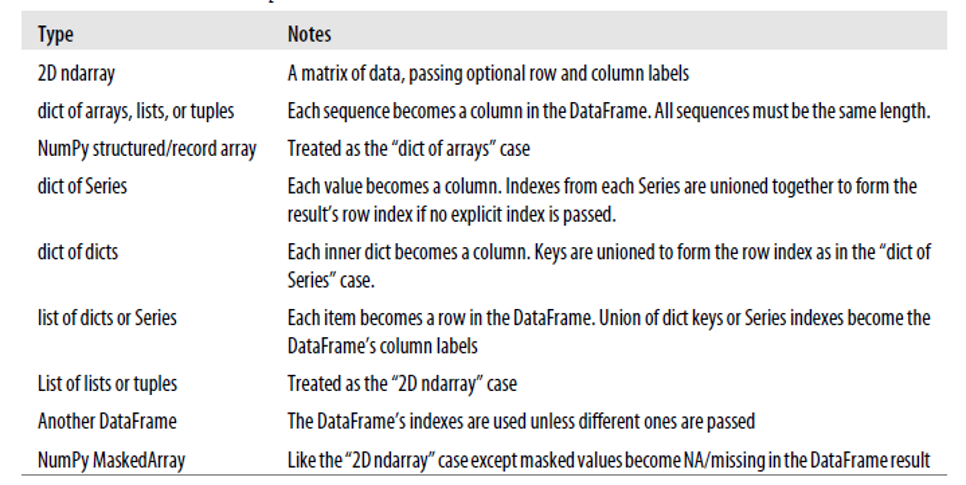
\includegraphics[width=0.9\linewidth,keepaspectratio]{pdf18}
\end{center}
\end{frame}


%%%%%%%%%%%%%%%%%%%%%%%%%%%%%%%%%%%%%%%%%%%%%%%%%%%%%%%%%%%%%%%%%%%%%%%%
\begin{frame}[fragile]
\frametitle{Exploring data frames}
\begin{lstlisting}
#List first 5 records
df.head()
\end{lstlisting}
\begin{center}
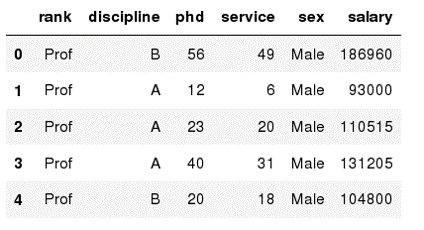
\includegraphics[width=0.5\linewidth,keepaspectratio]{pdf1}
\end{center}
\end{frame}

%%%%%%%%%%%%%%%%%%%%%%%%%%%%%%%%%%%%%%%%%%%%%%%%%%%%%%%%%%%%%%%%%%%%%%%%
\begin{frame}[fragile]
\frametitle{Exploring data frames}
\begin{lstlisting}
#List first 5 records
df.head()
\end{lstlisting}
\begin{center}
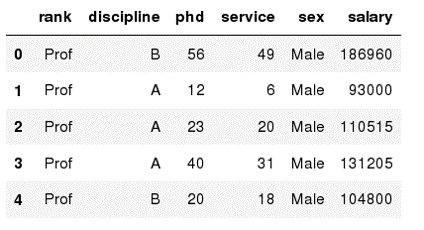
\includegraphics[width=0.5\linewidth,keepaspectratio]{pdf1}
\end{center}

\end{frame}



%%%%%%%%%%%%%%%%%%%%%%%%%%%%%%%%%%%%%%%%%%%%%%%%%%%%%%%%%%%%%%%%%%%%%%%%
\begin{frame}[fragile]
\frametitle{Hands-on exercises}
\begin{itemize}
\item Try to read the first 10, 20, 50 records.
\item Can you guess how to view the last few records?
\end{itemize}
\end{frame}
 
%%%%%%%%%%%%%%%%%%%%%%%%%%%%%%%%%%%%%%%%%%%%%%%%%%%%%%%%%%%%%%%%%%%%%%%%
\begin{frame}[fragile]
\frametitle{Data Frame data types}

\begin{center}
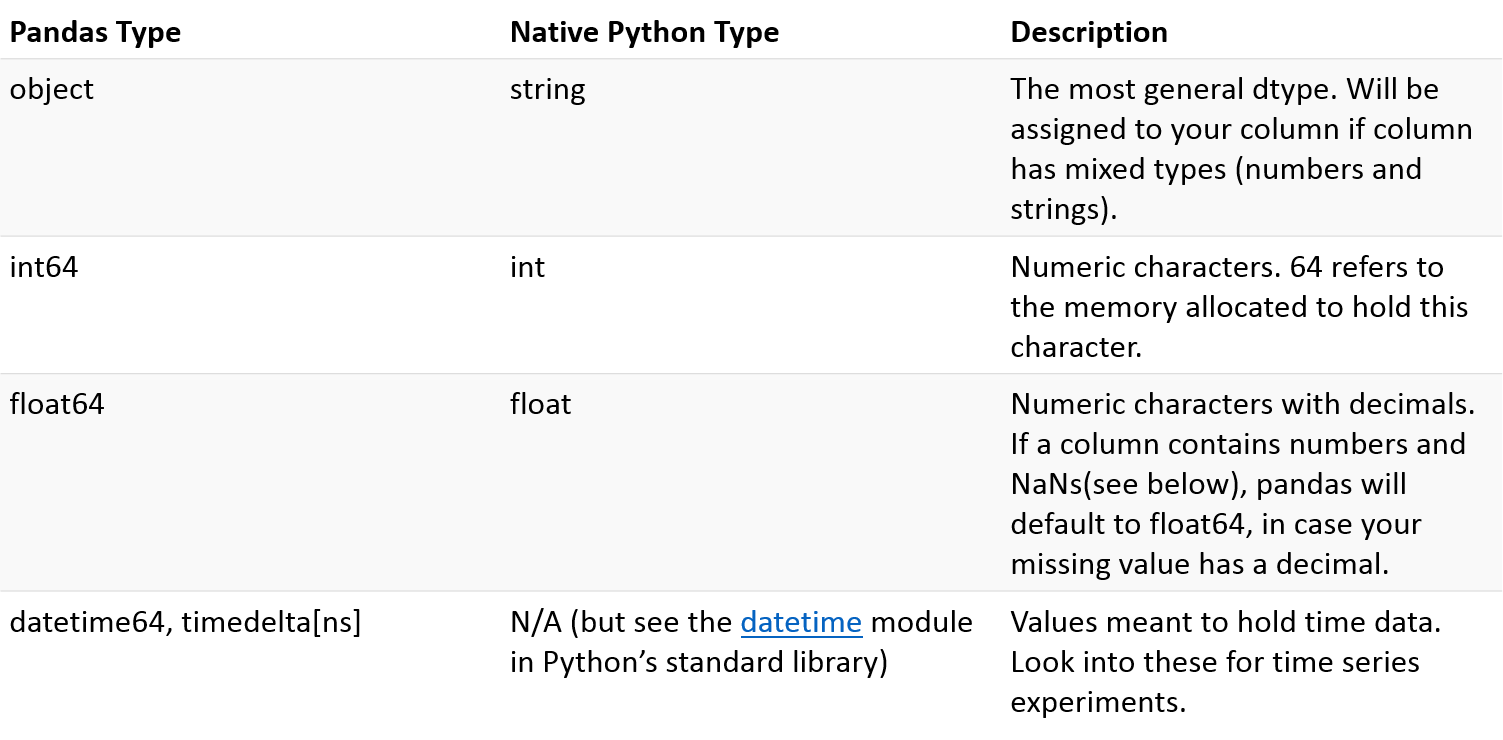
\includegraphics[width=\linewidth,keepaspectratio]{pdf2}
\end{center}

\end{frame}


%%%%%%%%%%%%%%%%%%%%%%%%%%%%%%%%%%%%%%%%%%%%%%%%%%%%%%%%%%%%%%%%%%%%%%%%
\begin{frame}[fragile]
\frametitle{Data Frame data types}
\begin{lstlisting}
#Check a particular column type
df['salary'].dtype

#Check types for all the columns
df.dtypes

rank     	object        
discipline  object
phd 		int64
service    int64
sex             object 
salary         int64
dtype: object
\end{lstlisting}
\end{frame}

%%%%%%%%%%%%%%%%%%%%%%%%%%%%%%%%%%%%%%%%%%%%%%%%%%%%%%%%%%%%%%%%%%%%%%%%
\begin{frame}[fragile]
\frametitle{Data Frames attributes}
Python objects have attributes.
\begin{center}
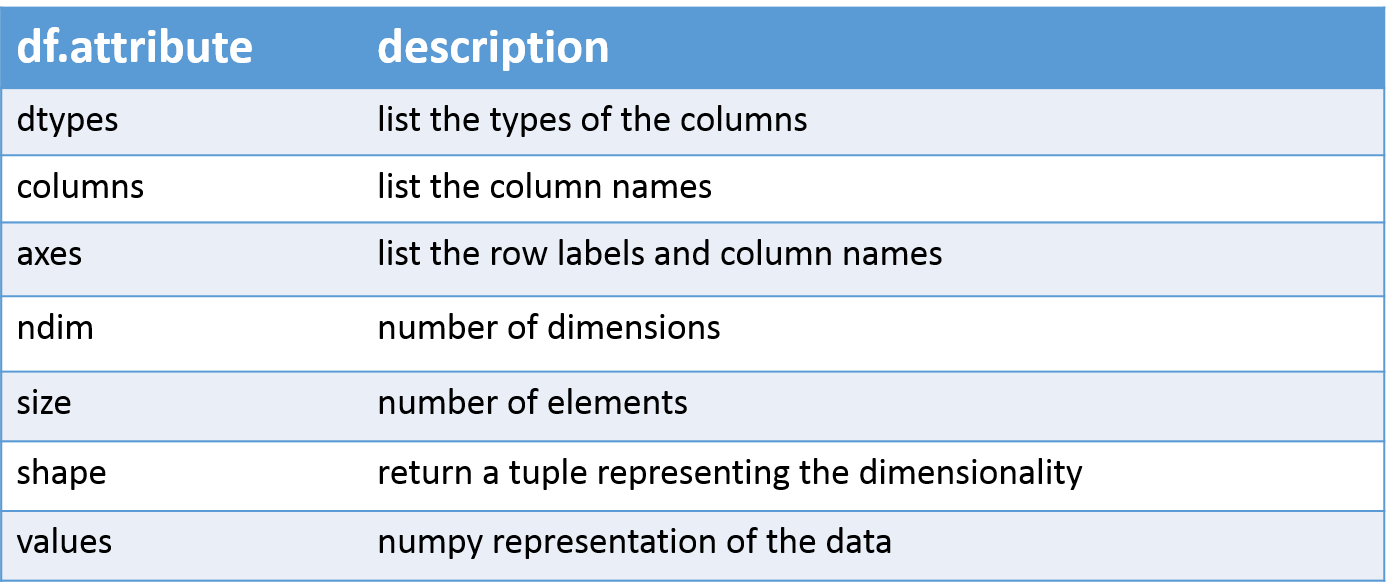
\includegraphics[width=\linewidth,keepaspectratio]{pdf3}
\end{center}

\end{frame}


%%%%%%%%%%%%%%%%%%%%%%%%%%%%%%%%%%%%%%%%%%%%%%%%%%%%%%%%%%%%%%%%%%%%%%%%
\begin{frame}[fragile]
\frametitle{Hands-on exercises}
\begin{itemize}
\item Find how many records this data frame has;
\item How many elements are there?     
\item What are the column names?
\item What types of columns we have in this data frame?
\end{itemize}

\end{frame}


%%%%%%%%%%%%%%%%%%%%%%%%%%%%%%%%%%%%%%%%%%%%%%%%%%%%%%%%%%%%%%%%%%%%%%%%
\begin{frame}[fragile]
\frametitle{Data Frames Methods}
Python objects have methods.
\begin{center}
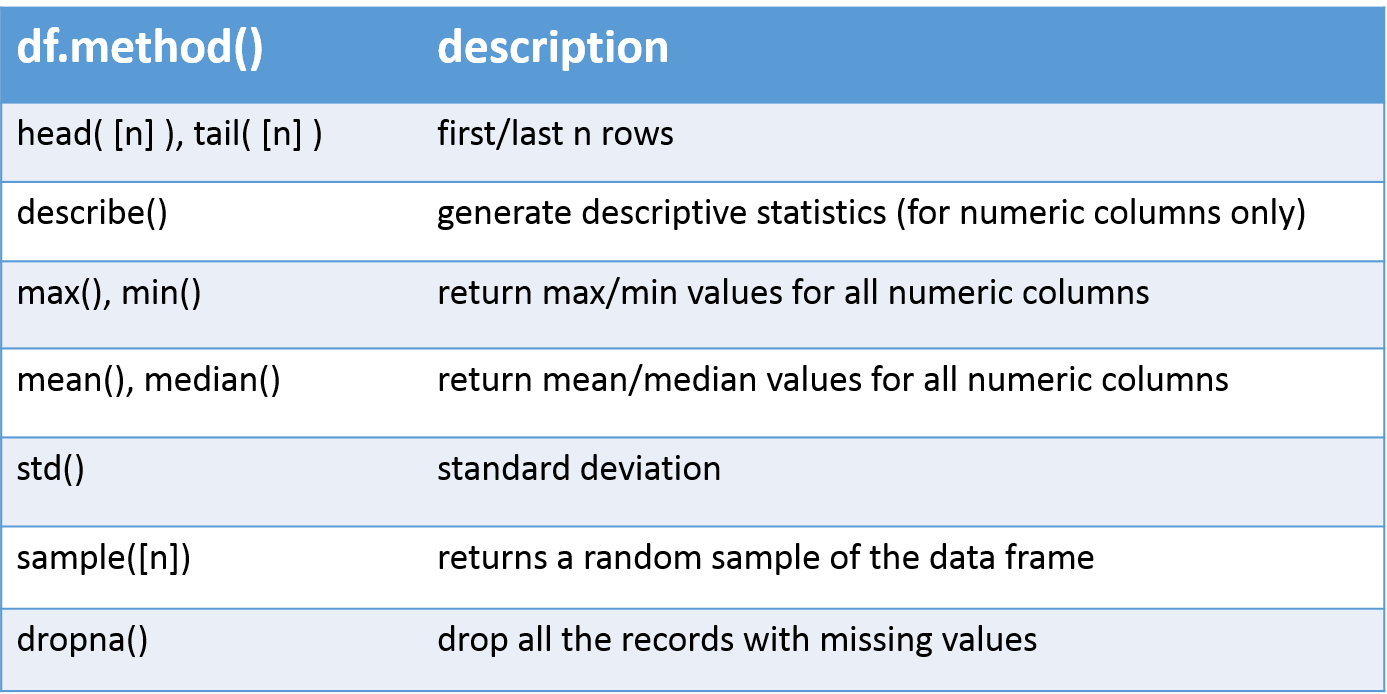
\includegraphics[width=\linewidth,keepaspectratio]{pdf4}
\end{center}

\end{frame}

%%%%%%%%%%%%%%%%%%%%%%%%%%%%%%%%%%%%%%%%%%%%%%%%%%%%%%%%%%%%%%%%%%%%%%%%
\begin{frame}[fragile]
\frametitle{Hands-on exercises}
\begin{itemize}
\item Give the summary for the numeric columns in the data-set
\item Calculate standard deviation for all numeric columns;
\item What are the mean values of the first 50 records in the data-set?   Hint: use head() method to subset the first 50 records and then calculate the mean
\end{itemize}

\end{frame}

%%%%%%%%%%%%%%%%%%%%%%%%%%%%%%%%%%%%%%%%%%%%%%%%%%%%%%%%%%%%%%%%%%%%%%%%
\begin{frame}[fragile]
\frametitle{Selecting a column in a Data Frame}
\begin{itemize}
\item Method 1:   Subset the data frame using column name:
                      df['col1']

\item Method 2:   Use the column name as an attribute:
                      df.col1

\end{itemize}

\end{frame}

%%%%%%%%%%%%%%%%%%%%%%%%%%%%%%%%%%%%%%%%%%%%%%%%%%%%%%%%%%%%%%%%%%%%%%%%
\begin{frame}[fragile]
\frametitle{Hands-on exercises}
\begin{itemize}
\item Calculate the basic statistics for the salary column;
\item Find how many values in the salary column (use count method);
\item Calculate the average salary
\end{itemize}

\end{frame}


%%%%%%%%%%%%%%%%%%%%%%%%%%%%%%%%%%%%%%%%%%%%%%%%%%%%%%%%%%%%%%%%%%%%%%%%
\begin{frame}[fragile]
\frametitle{Data Frame: filtering}
To subset the data we can apply Boolean indexing. This indexing is commonly known as a filter.  For example if we want to subset the rows in which the salary value is greater than \$120K: 

\begin{lstlisting}
#Calculate mean salary for each professor rank:
df_sub = df[ df['salary'] > 120000 ]

#Select only those rows that contain female professors:
df_f = df[ df['sex'] == 'Female' ]
\end{lstlisting}
\end{frame}

%%%%%%%%%%%%%%%%%%%%%%%%%%%%%%%%%%%%%%%%%%%%%%%%%%%%%%%%%%%%%%%%%%%%%%%%
\begin{frame}[fragile]
\frametitle{Data Frames: Slicing}
There are a number of ways to subset the Data Frame:

\begin{itemize}
\item one or more columns
\item one or more rows
\item a subset of rows and columns
\end{itemize}
Rows and columns can be selected by their position or label 

\end{frame}


%%%%%%%%%%%%%%%%%%%%%%%%%%%%%%%%%%%%%%%%%%%%%%%%%%%%%%%%%%%%%%%%%%%%%%%%
\begin{frame}[fragile]
\frametitle{Data Frames: Slicing}
When selecting one column, it is possible to use single set of brackets, but the resulting object will be  a Series (not a DataFrame): 
\begin{lstlisting}
#Select column salary:
df['salary']
\end{lstlisting}
When we need to select more than one column and/or make the output to be a DataFrame, we should use double brackets:
\begin{lstlisting}
#Select columns salary and rank:
df[['rank','salary']]

\end{lstlisting}
\end{frame}

%%%%%%%%%%%%%%%%%%%%%%%%%%%%%%%%%%%%%%%%%%%%%%%%%%%%%%%%%%%%%%%%%%%%%%%%
\begin{frame}[fragile]
\frametitle{Data Frames: Slicing}
If we need to select a range of rows, we can specify the range using ":" 

\begin{lstlisting}
#Select rows by their position:
df[10:20]
\end{lstlisting}
Notice that the first row has a position 0, and the last value in the range is omitted:
So for 0:10 range the first 10 rows are returned with the positions starting with 0 and ending with 9
\end{frame}


%%%%%%%%%%%%%%%%%%%%%%%%%%%%%%%%%%%%%%%%%%%%%%%%%%%%%%%%%%%%%%%%%%%%%%%%
\begin{frame}[fragile]
\frametitle{Data Frames: method loc}
To select a range of rows, using their labels, use method loc:

\begin{lstlisting}
#Select rows by their labels:
df_sub.loc[10:20,['rank','sex','salary']]
\end{lstlisting}
\begin{center}
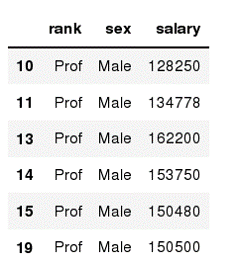
\includegraphics[width=0.35\linewidth,keepaspectratio]{pdf5}
\end{center}
\end{frame}

%%%%%%%%%%%%%%%%%%%%%%%%%%%%%%%%%%%%%%%%%%%%%%%%%%%%%%%%%%%%%%%%%%%%%%%%
\begin{frame}[fragile]
\frametitle{Data Frames: method iloc}
If we need to select a range of rows and/or columns, using their positions we can use method iloc:
\begin{lstlisting}
#Select rows by their labels:
df_sub.iloc[10:20,[0, 4, 5]]
\end{lstlisting}
\begin{center}
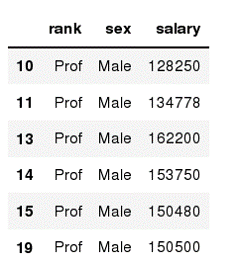
\includegraphics[width=0.35\linewidth,keepaspectratio]{pdf5}
\end{center}
\end{frame}

%%%%%%%%%%%%%%%%%%%%%%%%%%%%%%%%%%%%%%%%%%%%%%%%%%%%%%%%%%%%%%%%%%%%%%%%
\begin{frame}[fragile]
\frametitle{Data Frames: method iloc (summary)}
\begin{lstlisting}
df.iloc[0]  # First row of a data frame
df.iloc[i]  #(i+1)th row 
df.iloc[-1] # Last row 
df.iloc[:, 0]  # First column
df.iloc[:, -1] # Last column 
df.iloc[0:7]       #First 7 rows 
df.iloc[:, 0:2]    #First 2 columns
df.iloc[1:3, 0:2]  #Second through third rows and first 2 columns
df.iloc[[0,5], [1,3]]  #1st and 6th rows and 2nd and 4th columns
\end{lstlisting}

\end{frame}

%%%%%%%%%%%%%%%%%%%%%%%%%%%%%%%%%%%%%%%%%%%%%%%%%%%%%%%%%%%%%%%%%%%%%%%%
\begin{frame}[fragile]
\frametitle{Data Frames: Sorting}
We can sort the data by a value in the column. By default the sorting will occur in ascending order and a new data frame is return. 
\begin{lstlisting}
# Create a new data frame from the original sorted by the column Salary
df_sorted = df.sort_values( by ='service')
df_sorted.head()
\end{lstlisting}
\begin{center}
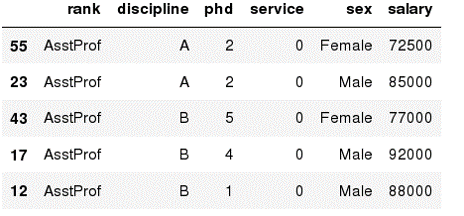
\includegraphics[width=0.65\linewidth,keepaspectratio]{pdf7}
\end{center}
\end{frame}

%%%%%%%%%%%%%%%%%%%%%%%%%%%%%%%%%%%%%%%%%%%%%%%%%%%%%%%%%%%%%%%%%%%%%%%%
\begin{frame}[fragile]
\frametitle{Data Frames: Sorting}
We can sort the data using 2 or more columns:
\begin{lstlisting}
df_sorted = df.sort_values( by =['service', 'salary'], ascending = [True, False])
df_sorted.head(10)
\end{lstlisting}
\begin{center}
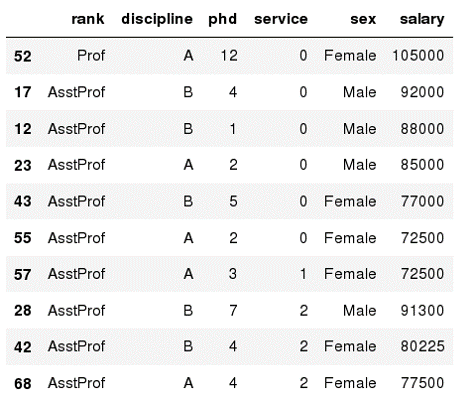
\includegraphics[width=0.5\linewidth,keepaspectratio]{pdf8}
\end{center}
\end{frame}

%%%%%%%%%%%%%%%%%%%%%%%%%%%%%%%%%%%%%%%%%%%%%%%%%%%%%%%%%%%%%%%%%%%%%%%%
\begin{frame}[fragile]
\frametitle{Data Frames: Basic Descriptive Statistics}
\begin{center}
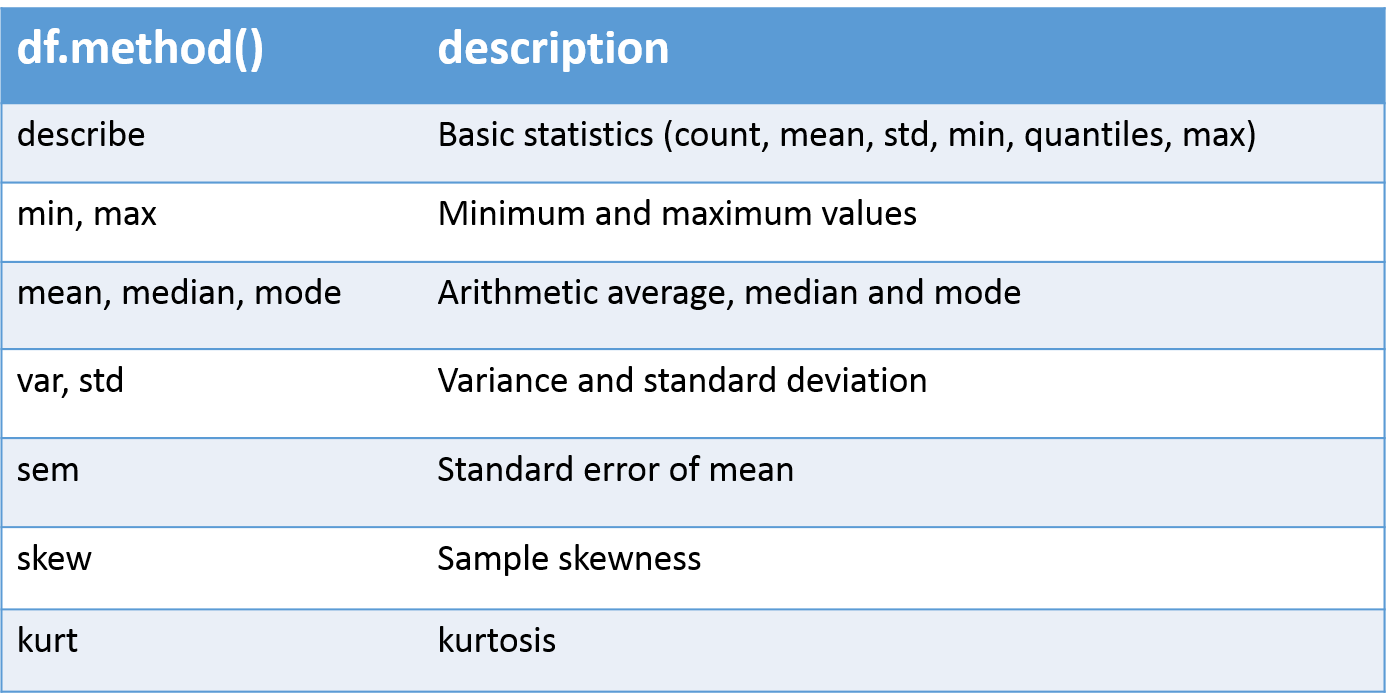
\includegraphics[width=\linewidth,keepaspectratio]{pdf11}
\end{center}
\end{frame}

%%%%%%%%%%%%%%%%%%%%%%%%%%%%%%%%%%%%%%%%%%%%%%%%%%%%%%%%%%%%%%%%%%%%%%%%
\begin{frame}[fragile]
\frametitle{Data Frames: Graphics to explore the data}
Seaborn package is built on matplotlib but provides high level interface for drawing attractive statistical graphics, similar to ggplot2 library in R. 
It specifically targets statistical data visualization

\begin{center}
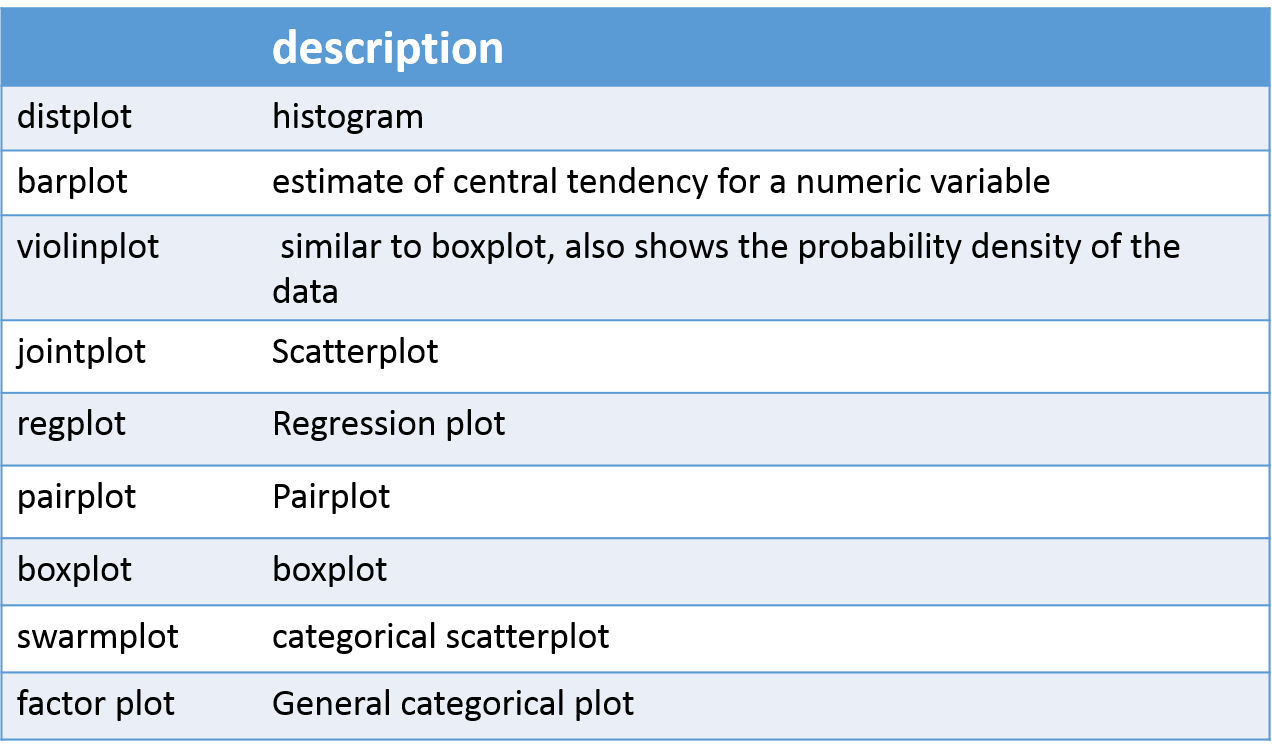
\includegraphics[width=0.8\linewidth,keepaspectratio]{pdf12}
\end{center}
\end{frame}


%%%%%%%%%%%%%%%%%%%%%%%%%%%%%%%%%%%%%%%%%%%%%%%%%%%%%%%%%%%%%%%%%%%%%%%%
\begin{frame}[fragile]
\frametitle{Data Frames: Boxplot example}
\begin{lstlisting}
df=DataFrame({'a': np.random.rand(1000), 'b': np.random.randn(1000, ), 'c': np.random.lognormal(size=(1000,))}
df.head()
a b c
0 0.356627 1.406655 3.288161
1 0.472792 -1.247858 2.499727
2 0.467848 0.406503 2.215045
3 0.341257 1.457440 0.390666
4 0.236013 0.026771 1.295106

df.boxplot()
plt.show()
\end{lstlisting}
\begin{center}
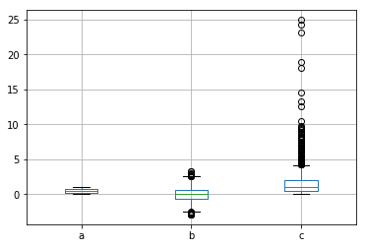
\includegraphics[width=0.4\linewidth,keepaspectratio]{pdf19}
\end{center}
\end{frame}

% %%%%%%%%%%%%%%%%%%%%%%%%%%%%%%%%%%%%%%%%%%%%%%%%%%%%%%%%%%%%%%%%%%%%%%%%
% \begin{frame}[fragile]
% \frametitle{Data Frames: Boxplot example 2}
% \begin{lstlisting}
% df2 = pd.read_csv('brfss.csv', index_col=0)
% df2.boxplot()
% plt.show()
% \end{lstlisting}
% \begin{center}
% 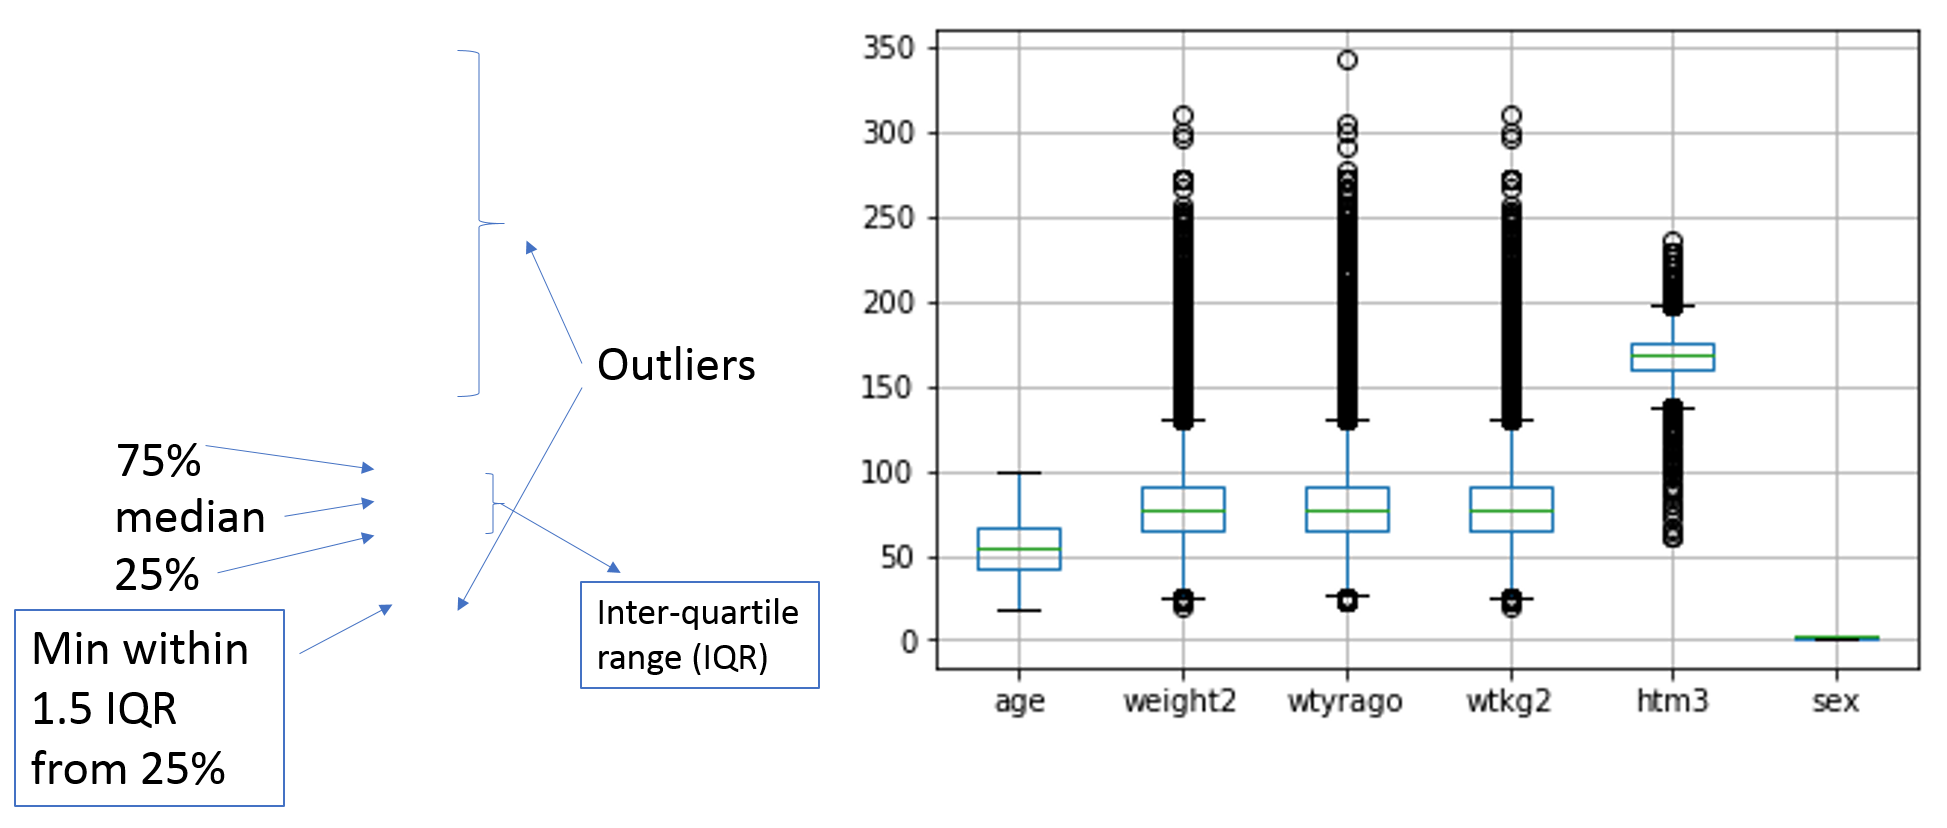
\includegraphics[width=0.8\linewidth,keepaspectratio]{pdf20}
% \end{center}
% \end{frame}


%%%%%%%%%%%%%%%%%%%%%%%%%%%%%%%%%%%%%%%%%%%%%%%%%%%%%%%%%%%%%%%%%%%%%%%%
\begin{frame}[fragile]
\frametitle{Data Frames: Hist}
\begin{lstlisting}
df2['weight2'].hist(bins=100)
plt.show()
\end{lstlisting}
\begin{center}
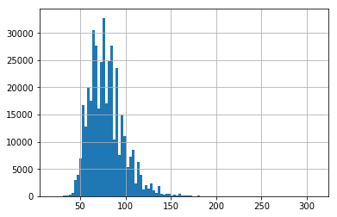
\includegraphics[width=0.8\linewidth,keepaspectratio]{pdf21}
\end{center}
\end{frame}


%%%%%%%%%%%%%%%%%%%%%%%%%%%%%%%%%%%%%%%%%%%%%%%%%%%%%%%%%%%%%%%%%%%%%%%%
\begin{frame}[fragile]
\frametitle{Data Frames: plot}
\begin{lstlisting}
df2['weight2'].hist(bins=100,normed=True); df2['weight2'].plot(kind='kde', style='k--')
plt.show()
\end{lstlisting}
\begin{center}
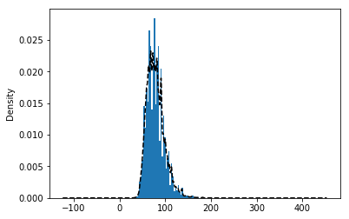
\includegraphics[width=0.8\linewidth,keepaspectratio]{pdf22}
\end{center}
\end{frame}

%%%%%%%%%%%%%%%%%%%%%%%%%%%%%%%%%%%%%%%%%%%%%%%%%%%%%%%%%%%%%%%%%%%%%%%%
\begin{frame}[fragile]
\frametitle{Data Frames: plot}
\begin{lstlisting}
df3 = DataFrame(np.random.randint(0, 10, (4, 3)), index=['A', 'B', 'C', 'D'], columns=['i', 'ii', 'iii'])
df3.plot()
plt.show()
\end{lstlisting}
\begin{center}
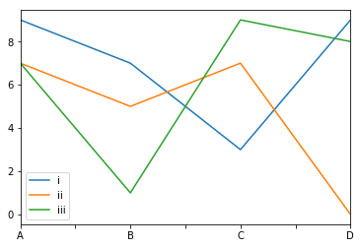
\includegraphics[width=0.6\linewidth,keepaspectratio]{pdf23}
\end{center}
\end{frame}

%%%%%%%%%%%%%%%%%%%%%%%%%%%%%%%%%%%%%%%%%%%%%%%%%%%%%%%%%%%%%%%%%%%%%%%%
\begin{frame}[fragile]
\frametitle{Data Frames: plot}
\begin{lstlisting}
df3.plot(kind='bar', stacked=True)
plt.show()
\end{lstlisting}
\begin{center}
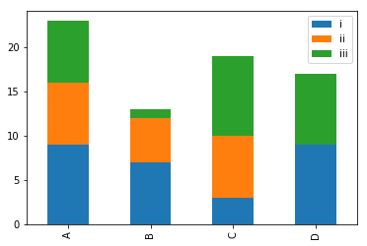
\includegraphics[width=0.6\linewidth,keepaspectratio]{pdf24}
\end{center}
\end{frame}


%%%%%%%%%%%%%%%%%%%%%%%%%%%%%%%%%%%%%%%%%%%%%%%%%%%%%%%%%%%%%%%%%%%%%%%%
\begin{frame}[fragile]
\frametitle{Data Frames: Function application and mapping}
DataFrame.apply(f) applies f to every column (default) or row
\begin{lstlisting}
In [1087]: frame
Out[1087]: 
c1 c2 c3
r1 0 1 2
r2 3 4 5
r3 6 7 8

In [1084]: def max_minus_min(x): return max(x)-min(x)
In [1085]: frame.apply(max_minus_min)
Out[1085]: 
c1 6
c2 6
c3 6

In [1086]: frame.apply(max_minus_min, axis=1)
Out[1086]: 
r1 2
r2 2
r3 2
\end{lstlisting}

\end{frame}



%%%%%%%%%%%%%%%%%%%%%%%%%%%%%%%%%%%%%%%%%%%%%%%%%%%%%%%%%%%%%%%%%%%%%%%%
\begin{frame}[fragile]
\frametitle{Data Frames: groupby}
Using ``group by'' method we can:
\begin{itemize}
\item Split the data into groups based on some criteria
\item Calculate statistics (or apply a function) to each group
\end{itemize}

\begin{lstlisting}
#Group data using rank
df_rank = df.groupby(['rank'])
#Calculate mean value for each numeric column per each group
df_rank.mean()
\end{lstlisting}

\begin{center}
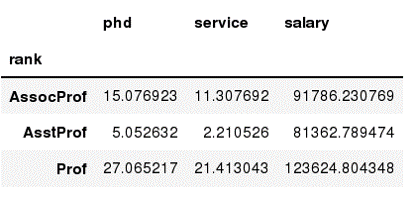
\includegraphics[width=0.5\linewidth,keepaspectratio]{pdf13}
\end{center}
\end{frame}

%%%%%%%%%%%%%%%%%%%%%%%%%%%%%%%%%%%%%%%%%%%%%%%%%%%%%%%%%%%%%%%%%%%%%%%%
\begin{frame}[fragile]
\frametitle{Data Frames: groupby}
Once groupby object is create we can calculate various statistics for each group:
\begin{lstlisting}
#Calculate mean salary for each professor rank:
df.groupby('rank')[['salary']].mean()
\end{lstlisting}

\begin{center}
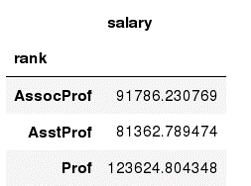
\includegraphics[width=0.3\linewidth,keepaspectratio]{pdf14}
\end{center}
Note: If single brackets are used to specify the column (e.g. salary), then the output is Pandas Series object. When double brackets are used the output is a Data Frame

\end{frame}

%%%%%%%%%%%%%%%%%%%%%%%%%%%%%%%%%%%%%%%%%%%%%%%%%%%%%%%%%%%%%%%%%%%%%%%%
\begin{frame}[fragile]
\frametitle{Data Frames: Aggregation}

Aggregation - computing a summary statistic about each group, i.e.
\begin{itemize}
\item compute group sums or means
\item compute group sizes/counts
\end{itemize}

Common aggregation functions:

\begin{itemize}
\item min, max
\item count, sum, prod
\item mean, median, mode, std, var
\end{itemize}

\end{frame}

%%%%%%%%%%%%%%%%%%%%%%%%%%%%%%%%%%%%%%%%%%%%%%%%%%%%%%%%%%%%%%%%%%%%%%%%
\begin{frame}[fragile]
\frametitle{Data Frames: Aggregation}
agg() method are useful when multiple statistics are computed per column:
\begin{lstlisting}
flights[['dep_delay','arr_delay']].agg(['min','mean','max'])
\end{lstlisting}

\begin{center}
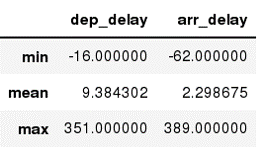
\includegraphics[width=0.35\linewidth,keepaspectratio]{pdf17}
\end{center}
\end{frame}

%%%%%%%%%%%%%%%%%%%%%%%%%%%%%%%%%%%%%%%%%%%%%%%%%%%%%%%%%%%%%%%%%%%%%%%%
\begin{frame}[fragile]
\frametitle{Data Frames: Missing Values}
Missing values are marked as NaN
\begin{lstlisting}
# Read a dataset with missing values
flights = pd.read_csv("http://rcs.bu.edu/examples/python/data_analysis/flights.csv")
# Select the rows that have at least one missing value
flights[flights.isnull().any(axis=1)].head()
\end{lstlisting}

\begin{center}
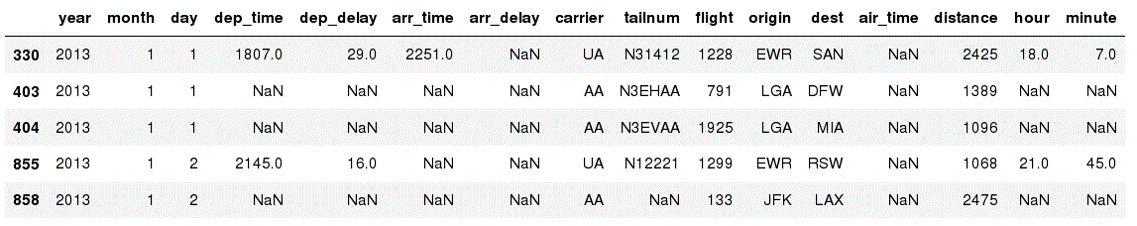
\includegraphics[width=0.9\linewidth,keepaspectratio]{pdf15}
\end{center}
\end{frame}

%%%%%%%%%%%%%%%%%%%%%%%%%%%%%%%%%%%%%%%%%%%%%%%%%%%%%%%%%%%%%%%%%%%%%%%%
\begin{frame}[fragile]
\frametitle{Data Frames: Missing Values}
There are a number of methods to deal with missing values in the data frame:
\begin{center}
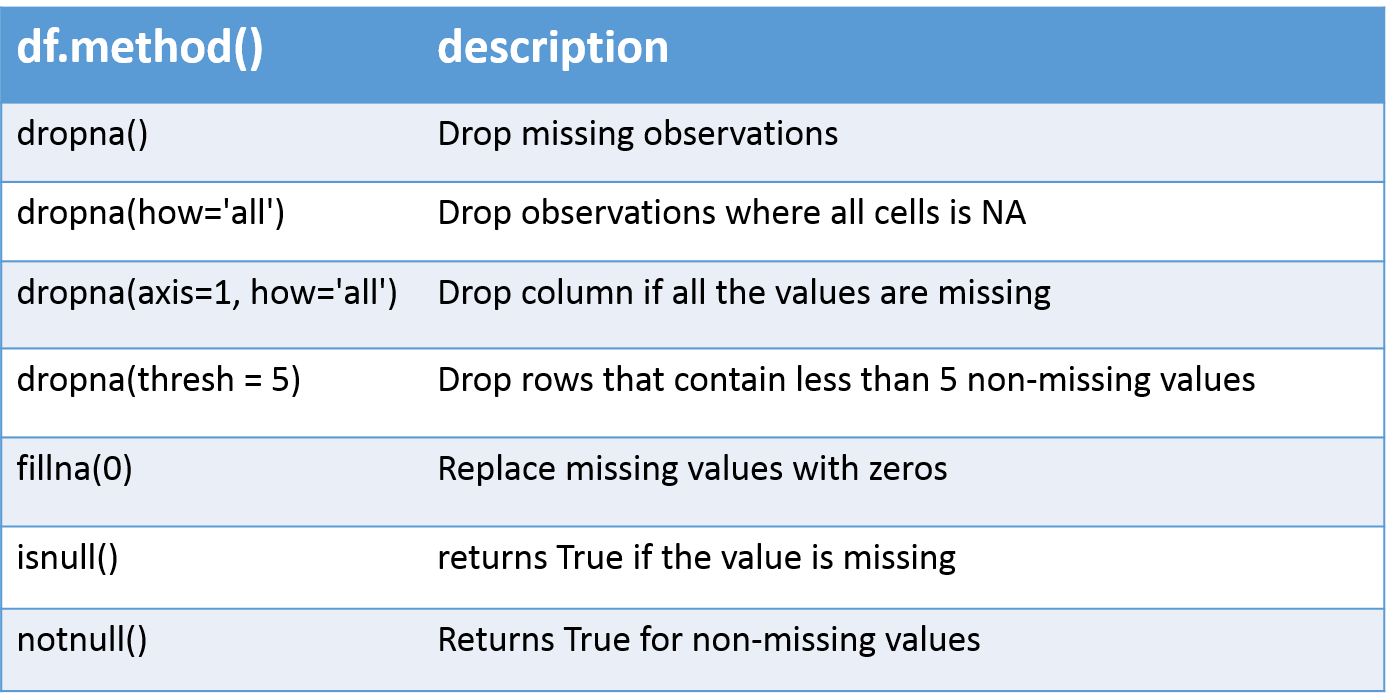
\includegraphics[width=0.9\linewidth,keepaspectratio]{pdf16}
\end{center}
\end{frame}

% %%%%%%%%%%%%%%%%%%%%%%%%%%%%%%%%%%%%%%%%%%%%%%%%%%%%%%%%%%%
% \begin{frame}[fragile]\frametitle{Creating Dataframes}
% Creating a DataFrame by passing a numpy array, with a datetime index and labeled columns:
% \begin{center}
% 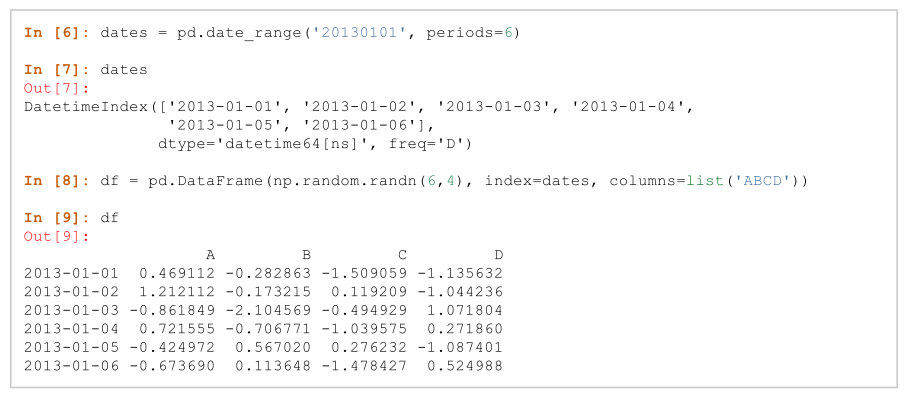
\includegraphics[width=\linewidth,keepaspectratio]{df1}
% \end{center}
% \end{frame}


% %%%%%%%%%%%%%%%%%%%%%%%%%%%%%%%%%%%%%%%%%%%%%%%%%%%%%%%%%%%
% \begin{frame}[fragile]\frametitle{Creating Dataframes}
% Creating a DataFrame by passing a dict of objects that can be converted to series-like.
% \begin{center}
% 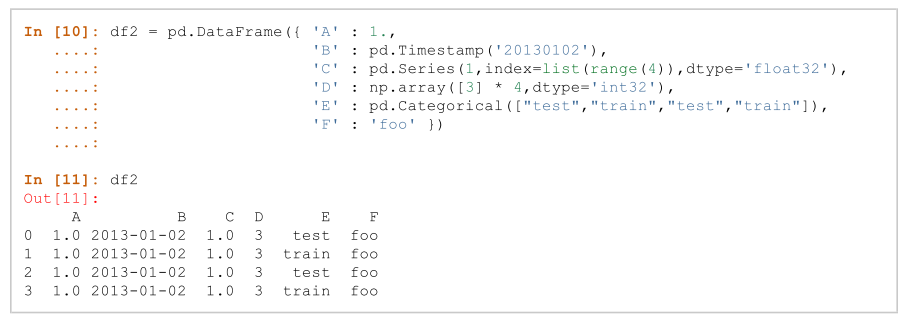
\includegraphics[width=\linewidth,keepaspectratio]{df2}
% \end{center}
% \end{frame}

% %%%%%%%%%%%%%%%%%%%%%%%%%%%%%%%%%%%%%%%%%%%%%%%%%%%%%%%%%%%
% \begin{frame}[fragile]\frametitle{Viewing Data}
% See the top \& bottom row s of the frame
% \begin{center}
% 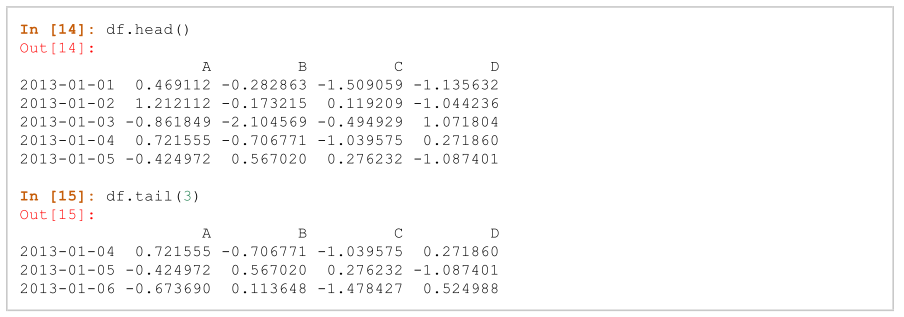
\includegraphics[width=\linewidth,keepaspectratio]{df3}
% \end{center}
% \end{frame}

% %%%%%%%%%%%%%%%%%%%%%%%%%%%%%%%%%%%%%%%%%%%%%%%%%%%%%%%%%%%
% \begin{frame}[fragile]\frametitle{Viewing Data}
% Display the index, columns, and the underlying numpy data
% \begin{center}
% 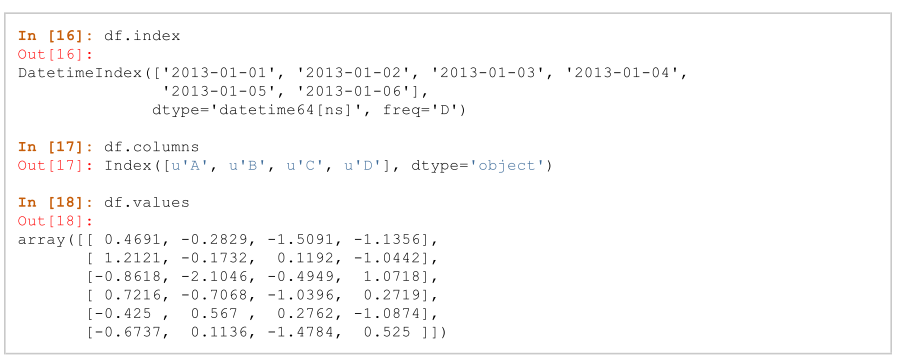
\includegraphics[width=\linewidth,keepaspectratio]{df4}
% \end{center}
% \end{frame}


% %%%%%%%%%%%%%%%%%%%%%%%%%%%%%%%%%%%%%%%%%%%%%%%%%%%%%%%%%%%
% \begin{frame}[fragile]\frametitle{Viewing Data}
% Describe show s a quick statistic summary of your data
% \begin{center}
% 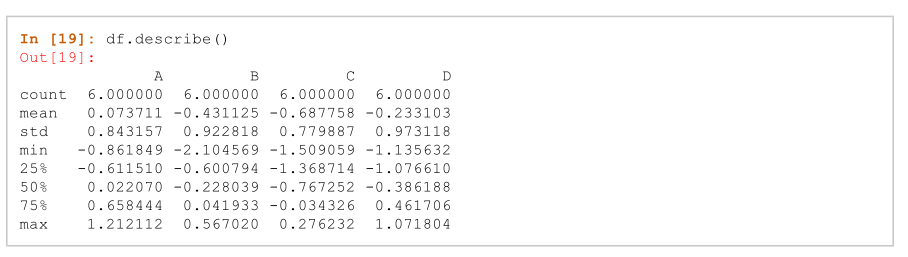
\includegraphics[width=\linewidth,keepaspectratio]{df5}
% \end{center}
% \end{frame}

% %%%%%%%%%%%%%%%%%%%%%%%%%%%%%%%%%%%%%%%%%%%%%%%%%%%%%%%%%%%
% \begin{frame}[fragile]\frametitle{Viewing Data}
% Sorting by an axis
% \begin{center}
% 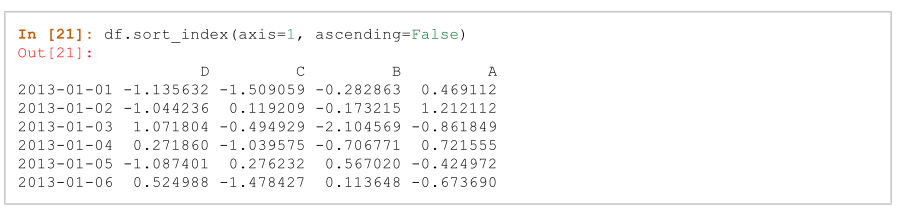
\includegraphics[width=\linewidth,keepaspectratio]{df6}
% \end{center}
% Sorting by values
% \begin{center}
% 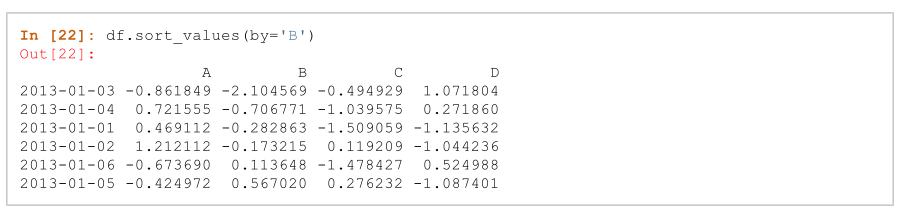
\includegraphics[width=\linewidth,keepaspectratio]{df7}
% \end{center}
% \end{frame}

% %%%%%%%%%%%%%%%%%%%%%%%%%%%%%%%%%%%%%%%%%%%%%%%%%%%%%%%%%%%
% \begin{frame}[fragile]\frametitle{Selection of  Data}
% Selecting a single column, which yields a Series, equivalent to df.A
% \begin{center}
% 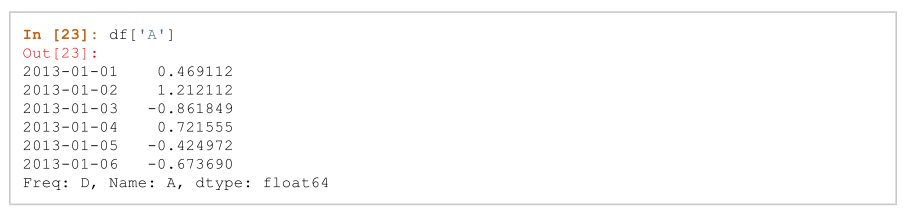
\includegraphics[width=\linewidth,keepaspectratio]{df8}
% \end{center}

% \end{frame}

% %%%%%%%%%%%%%%%%%%%%%%%%%%%%%%%%%%%%%%%%%%%%%%%%%%%%%%%%%%%
% \begin{frame}[fragile]\frametitle{Selection of  Data}
% Selecting via [], which slices the row s.
% \begin{center}
% 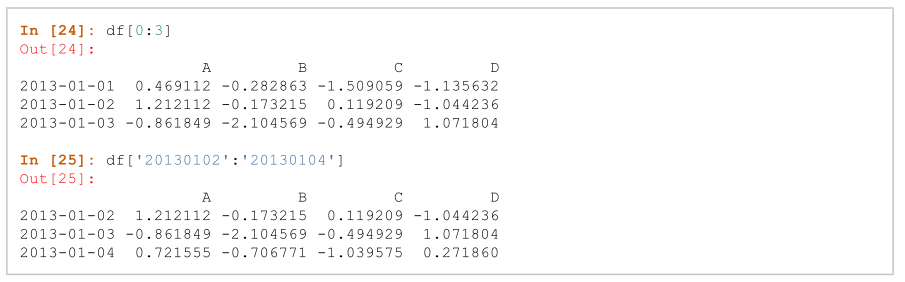
\includegraphics[width=\linewidth,keepaspectratio]{df9}
% \end{center}
% \end{frame}

% %%%%%%%%%%%%%%%%%%%%%%%%%%%%%%%%%%%%%%%%%%%%%%%%%%%%%%%%%%%
% \begin{frame}[fragile]\frametitle{Selection of  Data}
% Selecting on a multi-axis by label
% \begin{center}
% 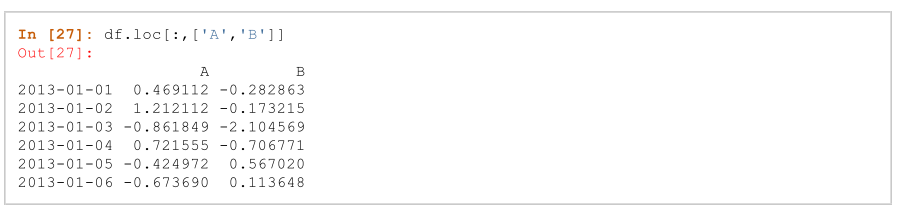
\includegraphics[width=\linewidth,keepaspectratio]{df10}
% \end{center}
% \end{frame}

% %%%%%%%%%%%%%%%%%%%%%%%%%%%%%%%%%%%%%%%%%%%%%%%%%%%%%%%%%%%
% \begin{frame}[fragile]\frametitle{Selection of  Data}
% By integer slices, acting similar to numpy/python
% \begin{center}
% 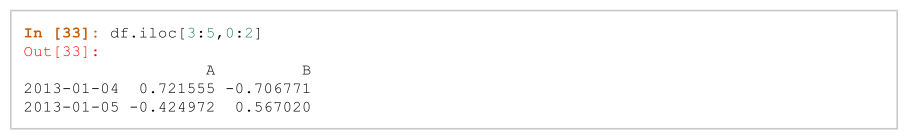
\includegraphics[width=\linewidth,keepaspectratio]{df11}
% \end{center}
% By lists of integer position locations, similar to the numpy/python style
% \begin{center}
% 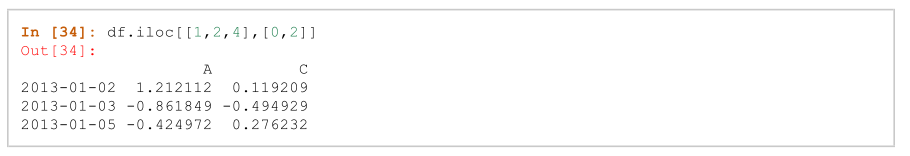
\includegraphics[width=\linewidth,keepaspectratio]{df12}
% \end{center}
% \end{frame}

% %%%%%%%%%%%%%%%%%%%%%%%%%%%%%%%%%%%%%%%%%%%%%%%%%%%%%%%%%%%
% \begin{frame}[fragile]\frametitle{ Boolean Indexing}
% Using a single column's values to select data.
% \begin{center}
% 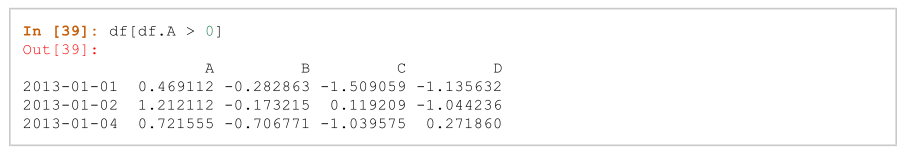
\includegraphics[width=\linewidth,keepaspectratio]{df13}
% \end{center}
% \end{frame}

% %%%%%%%%%%%%%%%%%%%%%%%%%%%%%%%%%%%%%%%%%%%%%%%%%%%%%%%%%%%
% \begin{frame}[fragile]\frametitle{ Missing Data}
% To drop any row s that have missing data.
% \begin{center}
% 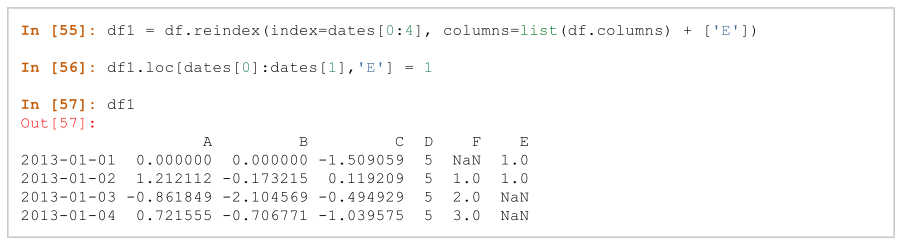
\includegraphics[width=\linewidth,keepaspectratio]{df14}
% \end{center}
% Filling missing data
% \begin{center}
% 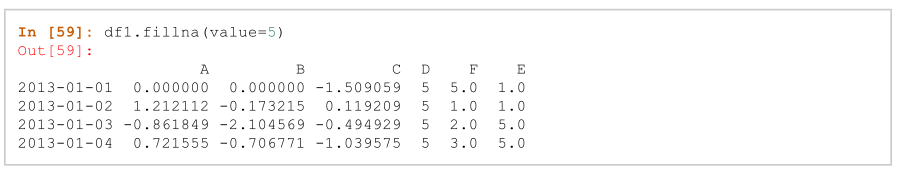
\includegraphics[width=\linewidth,keepaspectratio]{df15}
% \end{center}
% \end{frame}

% %%%%%%%%%%%%%%%%%%%%%%%%%%%%%%%%%%%%%%%%%%%%%%%%%%%%%%%%%%%
% \begin{frame}[fragile]\frametitle{ Stats}
% Operations in general exclude missing data.
% \begin{center}
% 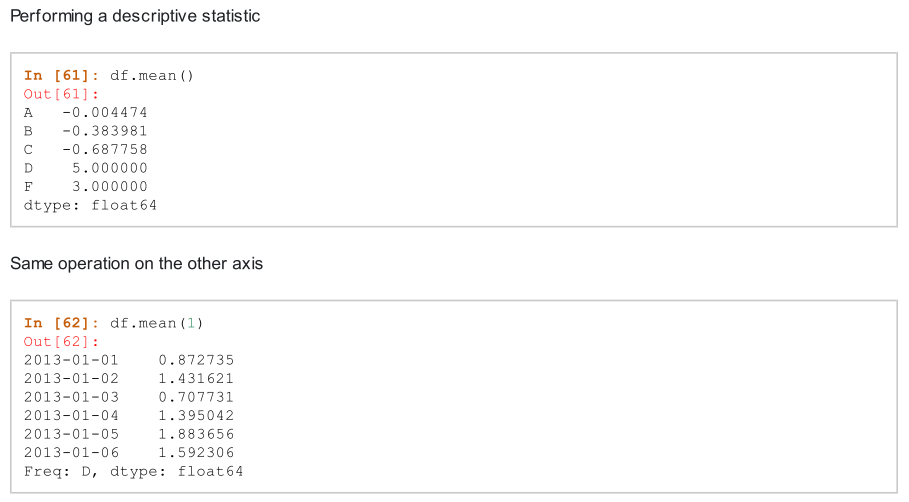
\includegraphics[width=\linewidth,keepaspectratio]{df16}
% \end{center}
% \end{frame}

% %%%%%%%%%%%%%%%%%%%%%%%%%%%%%%%%%%%%%%%%%%%%%%%%%%%%%%%%%%%
% \begin{frame}[fragile]\frametitle{ Apply}
% Applying functions to the data
% \begin{center}
% 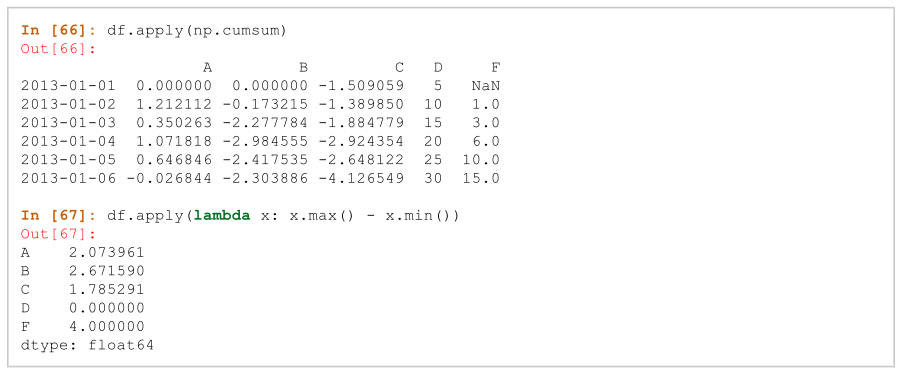
\includegraphics[width=\linewidth,keepaspectratio]{df17}
% \end{center}
% \end{frame}

%%%%%%%%%%%%%%%%%%%%%%%%%%%%%%%%%%%%%%%%%%%%%%%%%%%%%%%%%%%%%
%%\begin{frame}[fragile]\frametitle{ Case Study : MovieLens Dataset}
%%Contains 100,000 ratings made by 943 users on 1,682 movies.
%%\begin{lstlisting}
%%# pass in column names for each CSV
%%u_cols = ['user_id', 'age', 'sex', 'occupation', 'zip_code']
%%users = pd.read_csv('ml-100k/u.user', sep='|', names=u_cols)
%%
%%r_cols = ['user_id', 'movie_id', 'rating', 'unix_timestamp']
%%ratings = pd.read_csv('ml-100k/u.data', sep='\t', names=r_cols)
%%
%%# the movies file contains columns indicating the movie's genres
%%# let's only load the first five columns of the file with usecols
%%m_cols = ['movie_id', 'title', 'release_date', 'video_release_date', 'imdb_url']
%%movies = pd.read_csv('ml-100k/u.item', sep='|', names=m_cols, 
%%usecols=range(5))
%%\end{lstlisting}
%%\end{frame}
%%
%%
%%%%%%%%%%%%%%%%%%%%%%%%%%%%%%%%%%%%%%%%%%%%%%%%%%%%%%%%%%%%%
%%\begin{frame}[fragile]\frametitle{ Case Study : MovieLens Dataset}
%%\begin{lstlisting}
%%print(movies)
%%
%%Data columns (total 5 columns):
%%movie_id              1682  non-null values
%%title                 1682  non-null values
%%release_date          1681  non-null values
%%video_release_date    0  non-null values
%%imdb_url              1679  non-null values
%%dtypes: float64(1), int64(1), object(3)
%%\end{lstlisting}
%%\end{frame}
%%
%%
%%%%%%%%%%%%%%%%%%%%%%%%%%%%%%%%%%%%%%%%%%%%%%%%%%%%%%%%%%%%%
%%\begin{frame}[fragile]\frametitle{ Case Study : MovieLens Dataset}
%%\begin{itemize}
%%\item It is eveidently an instance of a DataFrame.
%%\item Each row was assigned an index of 0 to N-1, where N is the number of rows in the DataFrame. pandas will do this by default if an index is not specified. Don't worry, this can be changed later.
%%\item There are 1,682 rows (every row must have an index).
%%\item  dataset has five total columns, one of which isn't populated at all (video\_release\_date) and two that are missing some values (\texttt{release\_date} and \texttt{imdb\_url}).
%%\item The last line displays the datatypes of each column, but not necessarily in the corresponding order to the listed columns. You should use the dtypes method to get the datatype for each column.
%%\end{itemize}
%%\end{frame}
%%
%%%%%%%%%%%%%%%%%%%%%%%%%%%%%%%%%%%%%%%%%%%%%%%%%%%%%%%%%%%%%
%%\begin{frame}[fragile]\frametitle{ Case Study : MovieLens Dataset}
%%\begin{itemize}
%%\item It is eveidently an instance of a DataFrame.
%%\item Each row was assigned an index of 0 to N-1, where N is the number of rows in the DataFrame. pandas will do this by default if an index is not specified. Don't worry, this can be changed later.
%%\item There are 1,682 rows (every row must have an index).
%%\item  dataset has five total columns, one of which isn't populated at all (video\_release\_date) and two that are missing some values (\texttt{release\_date} and \texttt{imdb\_url}).
%%\item The last line displays the datatypes of each column, but not necessarily in the corresponding order to the listed columns. You should use the dtypes method to get the datatype for each column.
%%\end{itemize}
%%\end{frame}
%%
%%%%%%%%%%%%%%%%%%%%%%%%%%%%%%%%%%%%%%%%%%%%%%%%%%%%%%%%%%%%%
%%\begin{frame}[fragile]\frametitle{ Case Study : MovieLens Dataset}
%%\begin{lstlisting}
%%print(users.describe())
%%
%%user_id	age
%%count	 943.000000	 943.000000
%%mean	 472.000000	 34.051962
%%std	 272.364951	 12.192740
%%min	 1.000000	 7.000000
%%25%	 236.500000	 25.000000
%%50%	 472.000000	 31.000000
%%75%	 707.500000	 43.000000
%%max 943.000000 73.000000
%%\end{lstlisting}
%%Notice user\_id was included since it's numeric. Since this is an ID value, the stats for it don't really matter.
%%
%%We can quickly see the average age of our users is just above 34 years old, with the youngest being 7 and the oldest being 73. The median age is 31, with the youngest quartile of users being 25 or younger, and the oldest quartile being at least 43.
%%\end{frame}
%%
%%%%%%%%%%%%%%%%%%%%%%%%%%%%%%%%%%%%%%%%%%%%%%%%%%%%%%%%%%%%%
%%\begin{frame}[fragile]\frametitle{ Case Study : MovieLens Dataset}
%%\begin{lstlisting}
%%
%%print movies.head()
%%   movie_id              title release_date  video_release_date  \
%%0         1   Toy Story (1995)  01-Jan-1995                 NaN   
%%1         2   GoldenEye (1995)  01-Jan-1995                 NaN   
%%2         3  Four Rooms (1995)  01-Jan-1995                 NaN   
%%3         4  Get Shorty (1995)  01-Jan-1995                 NaN   
%%4         5     Copycat (1995)  01-Jan-1995                 NaN   
%%
%%                                            imdb_url  
%%0  http://us.imdb.com/M/title-exact?Toy%20Story%2...  
%%1  http://us.imdb.com/M/title-exact?GoldenEye%20(...  
%%2  http://us.imdb.com/M/title-exact?Four%20Rooms%...  
%%3  http://us.imdb.com/M/title-exact?Get%20Shorty%...  
%%4  http://us.imdb.com/M/title-exact?Copycat%20(1995)  
%%\end{lstlisting}
%%\end{frame}
%%
%%%%%%%%%%%%%%%%%%%%%%%%%%%%%%%%%%%%%%%%%%%%%%%%%%%%%%%%%%%%%
%%\begin{frame}[fragile]\frametitle{ Case Study : MovieLens Dataset}
%%\begin{lstlisting}
%%print movies.tail(3)
%%      movie_id                                      title release_date  \
%%1679      1680                       Sliding Doors (1998)  01-Jan-1998   
%%1680      1681                        You So Crazy (1994)  01-Jan-1994   
%%1681      1682  Scream of Stone (Schrei aus Stein) (1991)  08-Mar-1996   
%%
%%      video_release_date                                           imdb_url  
%%1679                 NaN      http://us.imdb.com/Title?Sliding+Doors+(1998)  
%%1680                 NaN  http://us.imdb.com/M/title-exact?You%20So%20Cr...  
%%1681                 NaN  http://us.imdb.com/M/title-exact?Schrei%20aus%...  
%%\end{lstlisting}
%%\end{frame}
%%
%%%%%%%%%%%%%%%%%%%%%%%%%%%%%%%%%%%%%%%%%%%%%%%%%%%%%%%%%%%%%
%%\begin{frame}[fragile]\frametitle{ Case Study : MovieLens Dataset}
%%You can think of a DataFrame as a group of Series that share an index (in this case the column headers). This makes it easy to select specific columns.
%%
%%Selecting a single column from the DataFrame will return a \texttt{Series} object.
%%\begin{lstlisting}
%%users['occupation'].head()
%%Out[38]:
%%0    technician
%%1         other
%%2        writer
%%3    technician
%%4         other
%%Name: occupation, dtype: object
%%\end{lstlisting}
%%\end{frame}
%%
%%
%%%%%%%%%%%%%%%%%%%%%%%%%%%%%%%%%%%%%%%%%%%%%%%%%%%%%%%%%%%%%
%%\begin{frame}[fragile]\frametitle{ Case Study : MovieLens Dataset}
%%To select multiple columns, simply pass a list of column names to the DataFrame, the output of which will be a DataFrame.
%%\begin{lstlisting}
%%print users[['age', 'zip_code']].head()
%%print '\n'
%%
%%# can also store in a variable to use later
%%columns_you_want = ['occupation', 'sex'] 
%%print users[columns_you_want].head()
%%   age zip_code
%%0   24    85711
%%1   53    94043
%%2   23    32067
%%3   24    43537
%%4   33    15213
%%
%%
%%   occupation sex
%%0  technician   M
%%1       other   F
%%2      writer   M
%%3  technician   M
%%4       other   F
%%\end{lstlisting}
%%\end{frame}
%%
%%
%%
%%
%%
%%%%%%%%%%%%%%%%%%%%%%%%%%%%%%%%%%%%%%%%%%%%%%%%%%%%%%%%%%%%%
%%\begin{frame}[fragile]\frametitle{ Case Study : MovieLens Dataset}
%%Row selection can be done multiple ways, but doing so by an individual index or boolean indexing are typically easiest.
%%\begin{lstlisting}
%%# users older than 25
%%print users[users.age > 25].head(3)
%%print '\n'
%%
%%# users aged 40 AND male
%%print users[(users.age == 40) & (users.sex == 'M')].head(3)
%%print '\n'
%%
%%# users younger than 30 OR female
%%print users[(users.sex == 'F') | (users.age < 30)].head(3)
%%   user_id  age sex occupation zip_code
%%1        2   53   F      other    94043
%%4        5   33   F      other    15213
%%5        6   42   M  executive    98101
%%
%%
%%     user_id  age sex  occupation zip_code
%%18        19   40   M   librarian    02138
%%82        83   40   M       other    44133
%%115      116   40   M  healthcare    97232
%%
%%
%%   user_id  age sex  occupation zip_code
%%0        1   24   M  technician    85711
%%1        2   53   F       other    94043
%%2        3   23   M      writer    32067
%%\end{verbatim}
%%\end{framed}
%%
%%
%%
%%
%%%%%%%%%%%%%%%%%%%%%%%%%%%%%%%%%%%%%%%%%%%%%%%%%%%%%%%%%%%%%
%%\begin{frame}[fragile]\frametitle{ Case Study : MovieLens Dataset}
%%Since our index is kind of meaningless right now, let's set it to the userid\_ using the set\_index method. By default, set\_index returns a new DataFrame, so you'll have to specify if you'd like the changes to occur in place.
%%
%%This has confused me in the past, so look carefully at the code and output below.
%%\begin{lstlisting}
%%print users.set_index('user_id').head()
%%print '\n'
%%
%%print users.head()
%%print "\n^^^ I didn't actually change the DataFrame. ^^^\n"
%%
%%with_new_index = users.set_index('user_id')
%%print with_new_index.head()
%%print "\n^^^ set_index actually returns a new DataFrame. ^^^\n"
%%         age sex  occupation zip_code
%%user_id                              
%%1         24   M  technician    85711
%%2         53   F       other    94043
%%3         23   M      writer    32067
%%4         24   M  technician    43537
%%5         33   F       other    15213
%%\end{lstlisting}
%%\end{frame}
%%
%%
%%%%%%%%%%%%%%%%%%%%%%%%%%%%%%%%%%%%%%%%%%%%%%%%%%%%%%%%%%%%%
%%\begin{frame}[fragile]\frametitle{ Case Study : MovieLens Dataset}
%%\begin{lstlisting}
%%   user_id  age sex  occupation zip_code
%%0        1   24   M  technician    85711
%%1        2   53   F       other    94043
%%2        3   23   M      writer    32067
%%3        4   24   M  technician    43537
%%4        5   33   F       other    15213
%%
%%^^^ I didn't actually change the DataFrame. ^^^
%%
%%         age sex  occupation zip_code
%%user_id                              
%%1         24   M  technician    85711
%%2         53   F       other    94043
%%3         23   M      writer    32067
%%4         24   M  technician    43537
%%5         33   F       other    15213
%%
%%^^^ set_index actually returns a new DataFrame. ^^^
%%\end{lstlisting}
%%\end{frame}
%%
%%
%%
%%
%%
%%%%%%%%%%%%%%%%%%%%%%%%%%%%%%%%%%%%%%%%%%%%%%%%%%%%%%%%%%%%%
%%\begin{frame}[fragile]\frametitle{ Case Study : MovieLens Dataset}
%%If you want to modify your existing DataFrame, use the inplace parameter.
%%\begin{lstlisting}
%%users.set_index('user_id', inplace=True)
%%print users.head()
%%         age sex  occupation zip_code
%%user_id                              
%%1         24   M  technician    85711
%%2         53   F       other    94043
%%3         23   M      writer    32067
%%4         24   M  technician    43537
%%5         33   F       other    15213
%%\end{lstlisting}
%%\end{frame}
%%
%%
%%
%%
%%%%%%%%%%%%%%%%%%%%%%%%%%%%%%%%%%%%%%%%%%%%%%%%%%%%%%%%%%%%%
%%\begin{frame}[fragile]\frametitle{ Case Study : MovieLens Dataset}
%%Notice that we've lost the default pandas 0-based index and moved the user\_id into its place. We can select rows based on the index using the ix method.
%%\begin{lstlisting}
%%print users.ix[99]
%%print '\n'
%%print users.ix[[1, 50, 300]]
%%age                20
%%sex                 M
%%occupation    student
%%zip_code        63129
%%Name: 99, dtype: object
%%
%%
%%     age sex  occupation zip_code
%%1     24   M  technician    85711
%%50    21   M      writer    52245
%%300   26   F  programmer    55106
%%\end{lstlisting}
%%\end{frame}
%%
%%
%%
%%%%%%%%%%%%%%%%%%%%%%%%%%%%%%%%%%%%%%%%%%%%%%%%%%%%%%%%%%%%%
%%\begin{frame}[fragile]\frametitle{ Case Study : MovieLens Dataset}
%%If we realize later that we liked the old pandas default index, we can just \texttt{reset\_index}. The same rules for inplace apply.
%%\begin{lstlisting}
%%users.reset_index(inplace=True)
%%print users.head()
%%   user_id  age sex  occupation zip_code
%%0        1   24   M  technician    85711
%%1        2   53   F       other    94043
%%2        3   23   M      writer    32067
%%3        4   24   M  technician    43537
%%4        5   33   F       other    15213
%%\end{lstlisting}
%%\end{frame}

%%%%%%%%%%%%%%%%%%%%%%%%%%%%%%%%%%%%%%%%%%%%%%%%%%%%%%%%%%%
\begin{frame}[fragile]\frametitle{ Pandas (Recap)}
\begin{itemize}
\item Working with CSV and Excel files using Pandas
\item Working with Pandas Dataframe
\begin{itemize}
\item Add a column to a dataframe
\item Remove a column from a dataframe
\item Subsetting a dataframe
\item Grouping a dataframe
\item Plotting
\end{itemize}
There are, of course, may more things that we can do with Pandas dataframes. Thats for you to explore.
\end{itemize}
\end{frame}
